\documentclass[11pt,border=2mm,tikz]{standalone}
\usepackage{csquotes}
\usepackage[backend=biber,style=numeric,sorting=none]{biblatex}

\providecommand{\FigScale}{1}

\usetikzlibrary{positioning, arrows.meta, fit, calc, backgrounds}

\definecolor{IBM5}{HTML}{ffb000}

\begin{document}
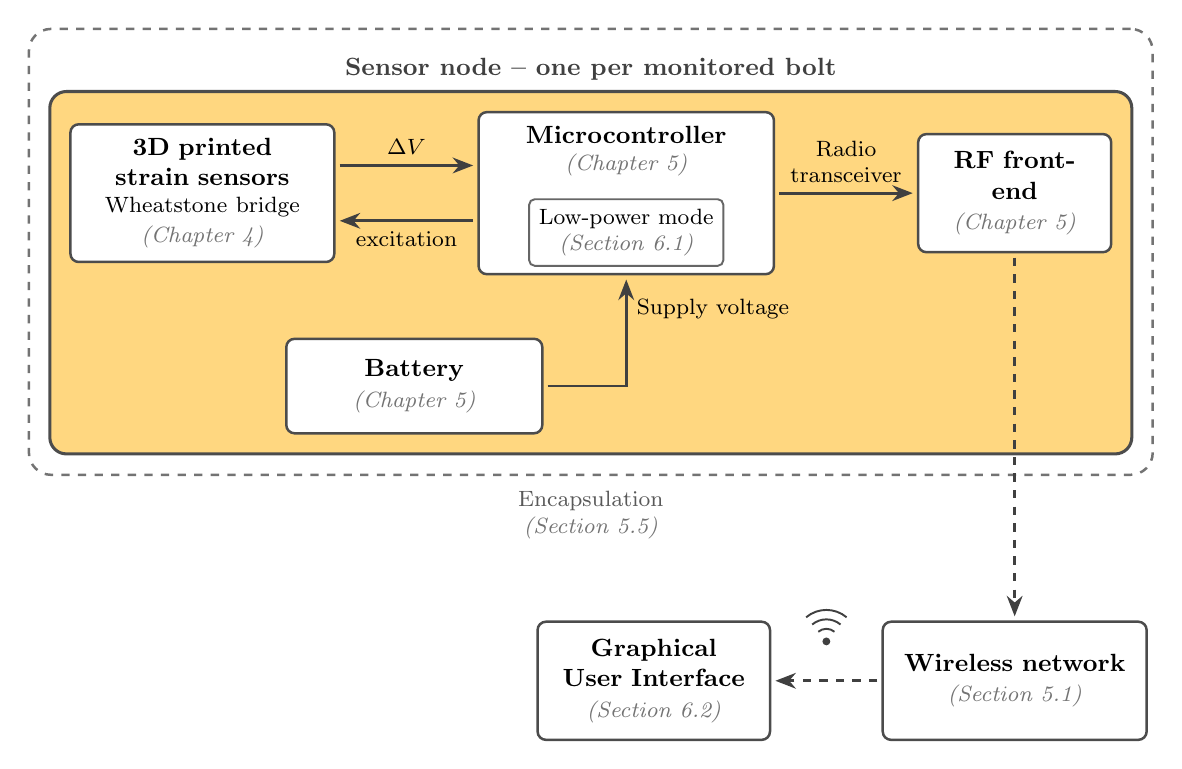
\begin{tikzpicture}[
  scale=\FigScale, transform shape,
  font=\small,
  block/.style={draw=black!70, line width=0.9pt, rounded corners=3pt, fill=white,
                align=center, minimum height=1.5cm, inner sep=5pt},
  sig/.style={-{Stealth[length=2.6mm, width=2mm]}, line width=1pt, draw=black!75,
              shorten <=1.5pt, shorten >=1.5pt},
  pwr/.style={-{Stealth[length=2.2mm, width=1.8mm]}, line width=0.9pt, draw=black!60,
              dashed, shorten <=1.5pt, shorten >=1.5pt}
]

\node[block, text width=3.0cm] (bridge)
  {\textbf{3D printed strain sensors}\\
   \footnotesize Wheatstone bridge\\
   {\footnotesize\itshape\color{black!55}(Chapter 4)}};

\node[block, right=1.8cm of bridge, text width=3.4cm] (mcu)
  {\textbf{Microcontroller}\\[1cm]
   {\footnotesize\strut}};

\node[font=\footnotesize\itshape, text=black!55, inner sep=0pt]
  at ([xshift=0cm, yshift=1.4cm]mcu.south) {(Chapter 5)};

\node[draw=black!60, line width=0.7pt, rounded corners=2pt, fill=white, align=center,
      font=\footnotesize, inner sep=3.5pt] (lpm) at ([yshift=-0.5cm]mcu.center)
  {Low-power mode\\
   {\itshape\color{black!55}(Section 6.1)}};

\node[block, text width=2.9cm, minimum height=1.2cm]
  (bat) at ($(bridge)!0.5!(mcu)+(0,-2.45)$)
  {\textbf{Battery}\\
   {\footnotesize\itshape\color{black!55}(Chapter 5)}};

\node[block, right=1.8cm of mcu, text width=2.1cm] (rf)
  {\textbf{RF front-end}\\
   {\footnotesize\itshape\color{black!55}(Chapter 5)}};



\begin{scope}[on background layer]
\node[draw=black!70, line width=1.1pt, rounded corners=6pt, fill=IBM5!50,
      inner sep=7pt, fit=(bridge)(mcu)(bat)(rf)] (nodebox) {};
\end{scope}
\node[anchor=south, font=\small\bfseries, text=black!75]
  (nodetitle) at (nodebox.north) {Sensor node -- one per monitored bolt};

\node[draw=black!55, dashed, line width=0.9pt, rounded corners=8pt, inner sep=7pt,
      fit=(nodebox)(nodetitle)] (encap) {};
\node[anchor=north, font=\footnotesize, text=black!65, align=center]
  at ([yshift=-2pt]encap.south)
  {Encapsulation\\
   {\itshape\color{black!55}(Section 5.5)}};

\node[block, text width=3.0cm] (net) at ([yshift=-2.6cm]encap.south -| rf.south)
  {\textbf{Wireless network}\\
   {\footnotesize\itshape\color{black!55}(Section 5.1)}};

\node[block, left=1.4cm of net, text width=2.6cm] (ha)
  {\textbf{Graphical User Interface}\\
   {\footnotesize\itshape\color{black!55}(Section 6.2)}};


\draw[sig] ([yshift=10pt]bridge.east) -- node[above, font=\footnotesize]{\(\Delta V\)}
           ([yshift=10pt]mcu.west);
\draw[sig] ([yshift=-10pt]mcu.west) -- node[below, font=\footnotesize]{excitation}
           ([yshift=-10pt]bridge.east);
\draw[sig] (bat.east) -| node[right, font=\footnotesize, pos=0.85]{Supply voltage} (mcu.south);
\draw[sig] (mcu.east) -- node[above, font=\footnotesize, align=center]{Radio\\transceiver} (rf.west);

\draw[sig, dashed] (rf.south) -- (net.north);
\draw[sig, dashed] (net.west) -- (ha.east);

\begin{scope}[shift={($(net.west)!0.5!(ha.east)+(0,0.5)$)}]
  \fill[black!75] (0,0) circle (0.05);
  \foreach \r in {0.16, 0.28, 0.40}
    \draw[black!75, line width=0.7pt] (50:\r) arc[start angle=50, end angle=130, radius=\r];
\end{scope}

\end{tikzpicture}
\end{document}
